%!TEX root=report.tex
\subsection{OLS}

The first part of the OLS analysis will look at the EWH at two specific locations. The second part will then focus on the entire world. The main purpose of the OLS analysis is to estimate the velocity and acceleration of the gravity changes.

\subsubsection{Selected locations}

The two selected locations are:
\begin{itemize}
\item Greenland ($63.5^\circ$ N, $49.5^\circ$ W)
\item South Pole ($74.5^\circ$ S, $87.5^\circ$ W)
\end{itemize}
\begin{figure}[H]
	\centering
	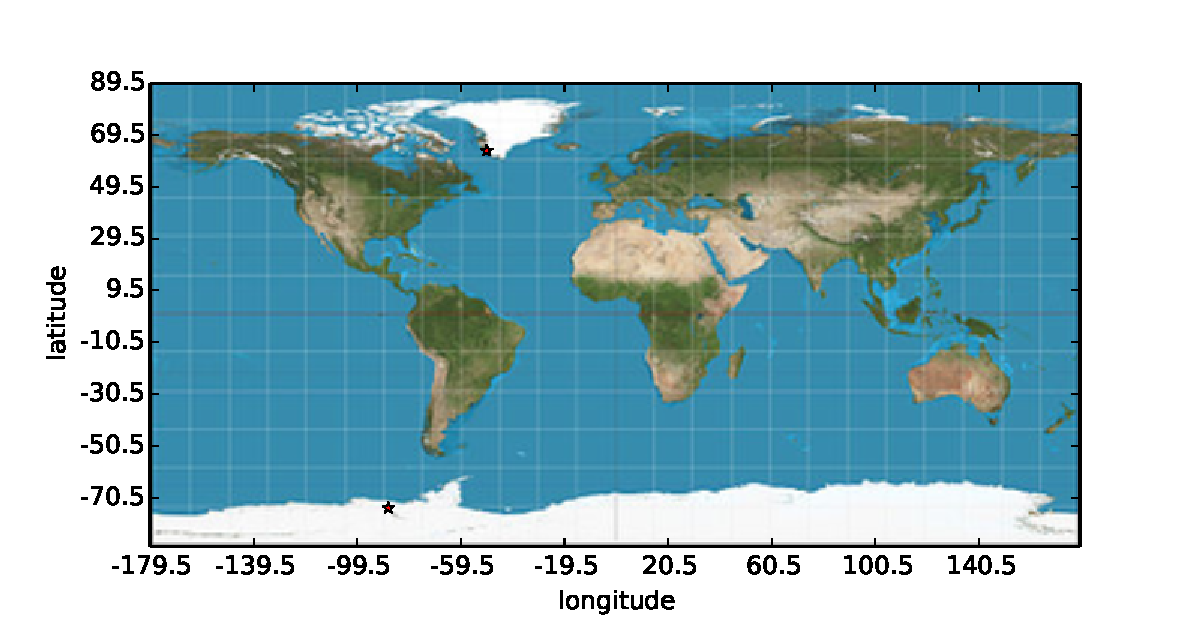
\includegraphics[height=6cm]{figures/ols-selected-map}
	\caption{The two selected locations, marked with a red star}
\end{figure}

\paragraph{Greenland}

At the west coast of Greenland is a strong period trend, caused by the the ice melting over the summer and reappearing over the winter. This trend is seen in Figure \ref{fig:ols-selected-0-fit}. In order to estimate the velocity and acceleration it's important that this trend is caught by the $\sin(\cdot)$ and $\cos(\cdot)$ terms in OLS regression.
\begin{figure}[H]
	\centering
	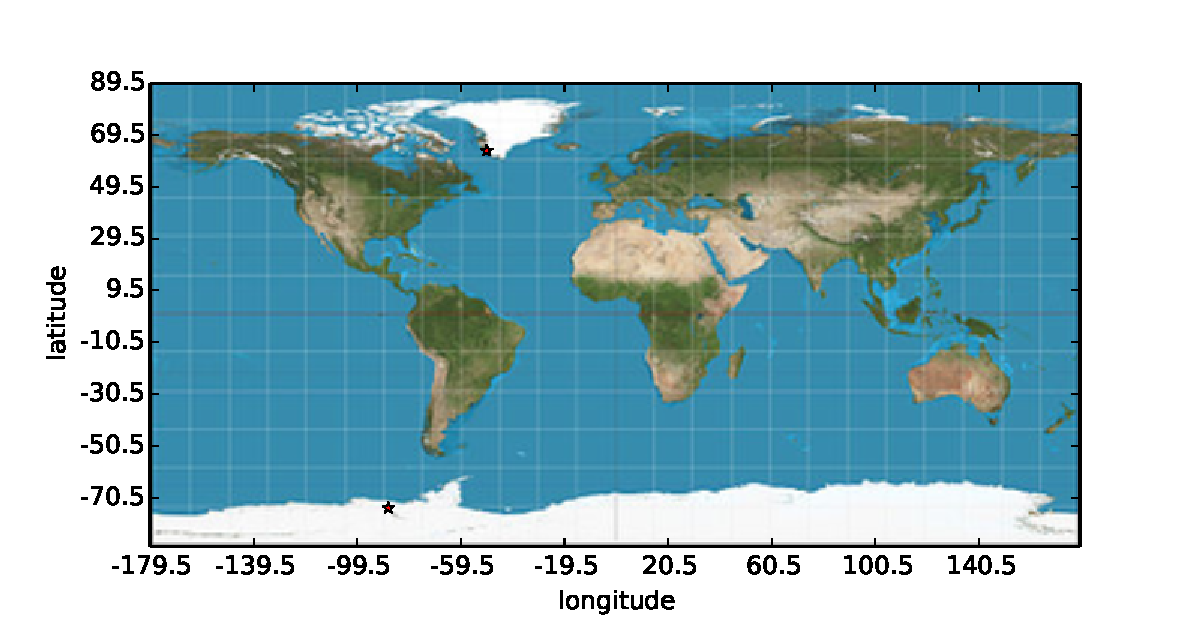
\includegraphics[width=\textwidth]{figures/ols-selected-0-fit}
	\caption{Messurements are blue, the OLS fit is red.}
	\label{fig:ols-selected-0-fit}
\end{figure}
 
From Figure \ref{fig:ols-selected-0-fit} it's seen that the period trend is caught by the model, however for some seasons (particular between 2008 and 2010) the fit is not very good. This is even more clear when looking at the residuals (Figure \ref{fig:ols-selected-0-residual}). From this it's clear that the residuals are far from white noise, which was one of the OLS assumptions.

\begin{figure}[H]
	\centering
	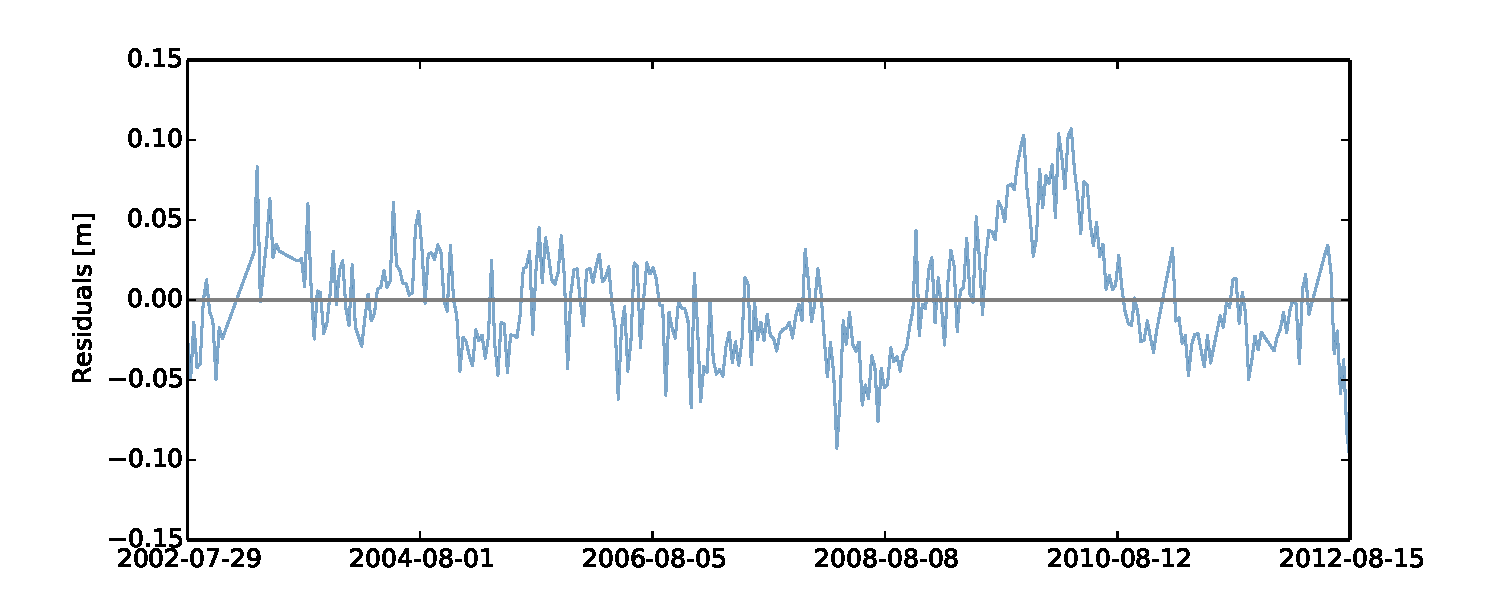
\includegraphics[width=\textwidth]{figures/ols-selected-0-residual}
	\caption{The OLS residuals are blue.}
	\label{fig:ols-selected-0-residual}
\end{figure}
